All results presented below can be reproduced by following a publicly
available
lab\footnote{\url{https://gitlab.inria.fr/VeRDi-project/madeus-journal}}.


%--------------------------------------
\subsection{Prototype implementation details}

\mad was implemented using \python. As illustrated in
Listings~\ref{codemdb}, \ref{codeapache} and~\ref{codeass}, users of
\mad declare a component by creating a class inheriting from the
internal \emph{Component} class, and containing a description of the
internal net (places and transtions) as well as actions associated
with transitions. These actions are \python functions that can perform
remote actions using SSH, Ansible or other tools. Users can then
create an assembly by extending the appropriate classes and listing
components and port connections. This assembly can then be executed
according to the semantics of \mad. The commissioning is over if the
only elements holding tokens are places without outgoing
transitions. The semantics is executed by attempting to apply each
rule on each component until this condition is met. When a
transition is fired, the corresponding \python function is executed in
a thread, which does not block the execution of the
semantics. Note that \python threads do not take advantage of hardware
parallelism capabilities, but because the functions usually run other
(possibly remote) processes to launch configuration commands, this is
not an issue. The $\terminaction$ rule can be executed for the
corresponding function when it has finished its execution.

% --------------------------------------
\subsection{Results}

Madeus is a model that relies on the description of a control
component for each software module to be deployed. It is a low-level
model, therefore the developer is responsible for the choices of
actions performed in the transitions as well as data and service
exchanges (\eg scp, VPN, REST API, etc.).  This section evaluates the
overhead introduced by the prototype of \mad as well as its
scalability when increasing the number of components and
transitions.
% SR: repetition
%Empty transitions are used to evaluate \mad independently
%of any specific transitions and additional overhead.
These experiments are dry runs, meaning that transitions do not
contain any code or command for which the execution time is unknown or
variable, and instead use sleep commands to simulate time-consuming
tasks. This allows us to measure the overhead introduced by the
prototype. In addition to this, the experiments presented in this
section are compared to the expected performance computed by the
prediction model detailed in Section~\ref{sec:perf_model}. This way,
we validate both the theoretical performance model compared to
reality, and the expected performance of the prototype on the set of
use cases.

% figures to add for assemblies
%Sequential

\begin{figure}[h]
  \begin{center}
    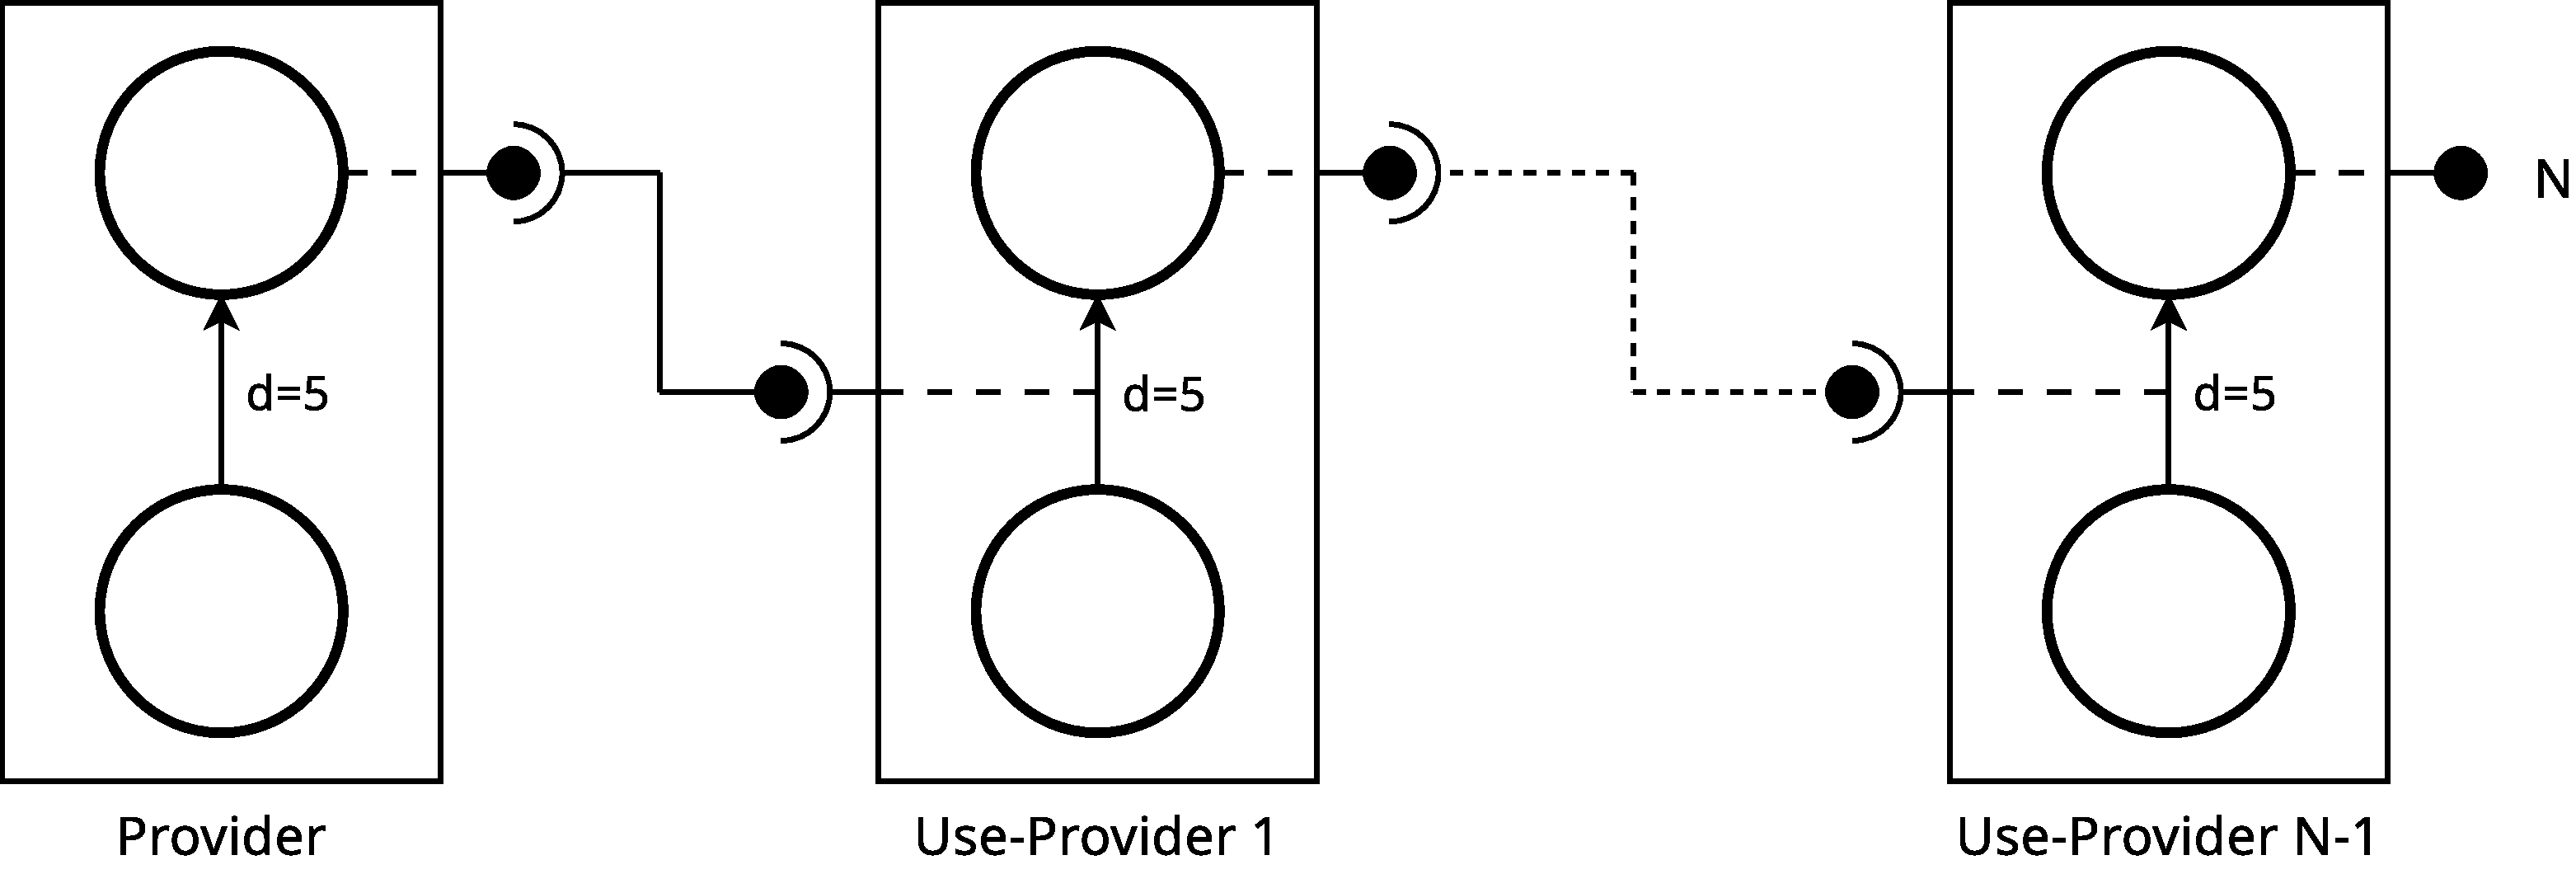
\includegraphics[width=0.4\textwidth]{./images/seq.pdf}
    \caption{The \mad sequential assembly of Benchmark (A), with N components. The dotted connection represents that $N-1$ other components exist in this assembly.}
    \label{fig:seq}
  \end{center}
\end{figure}

This evaluation is composed of three benchmarks illustrated in
Figures~\ref{fig:seq} and~\ref{fig:par}.
% first
The first benchmark, denoted (A), models a sequential \mad assembly,
depicted in Figure~\ref{fig:seq}. It is composed of one
\emph{provider} component made of a transition and two places, and
$N-1$ \emph{user-provider} components that are also composed of a
transition and two places, but where the transition uses the provide
port of the preceeding component. The components are connected in
a chain, resulting in sequential execution.
%The dry-run version of
%this assembly consists in transitions that do nothing besides wait for
%a fixed amount of time.
%The second version of this assembly features a transition that calls
%an ssh connection and waits for a fixed amount of time, similar as for
%the dry-run version, before finishing.

\begin{figure}[h]
  \begin{center}
    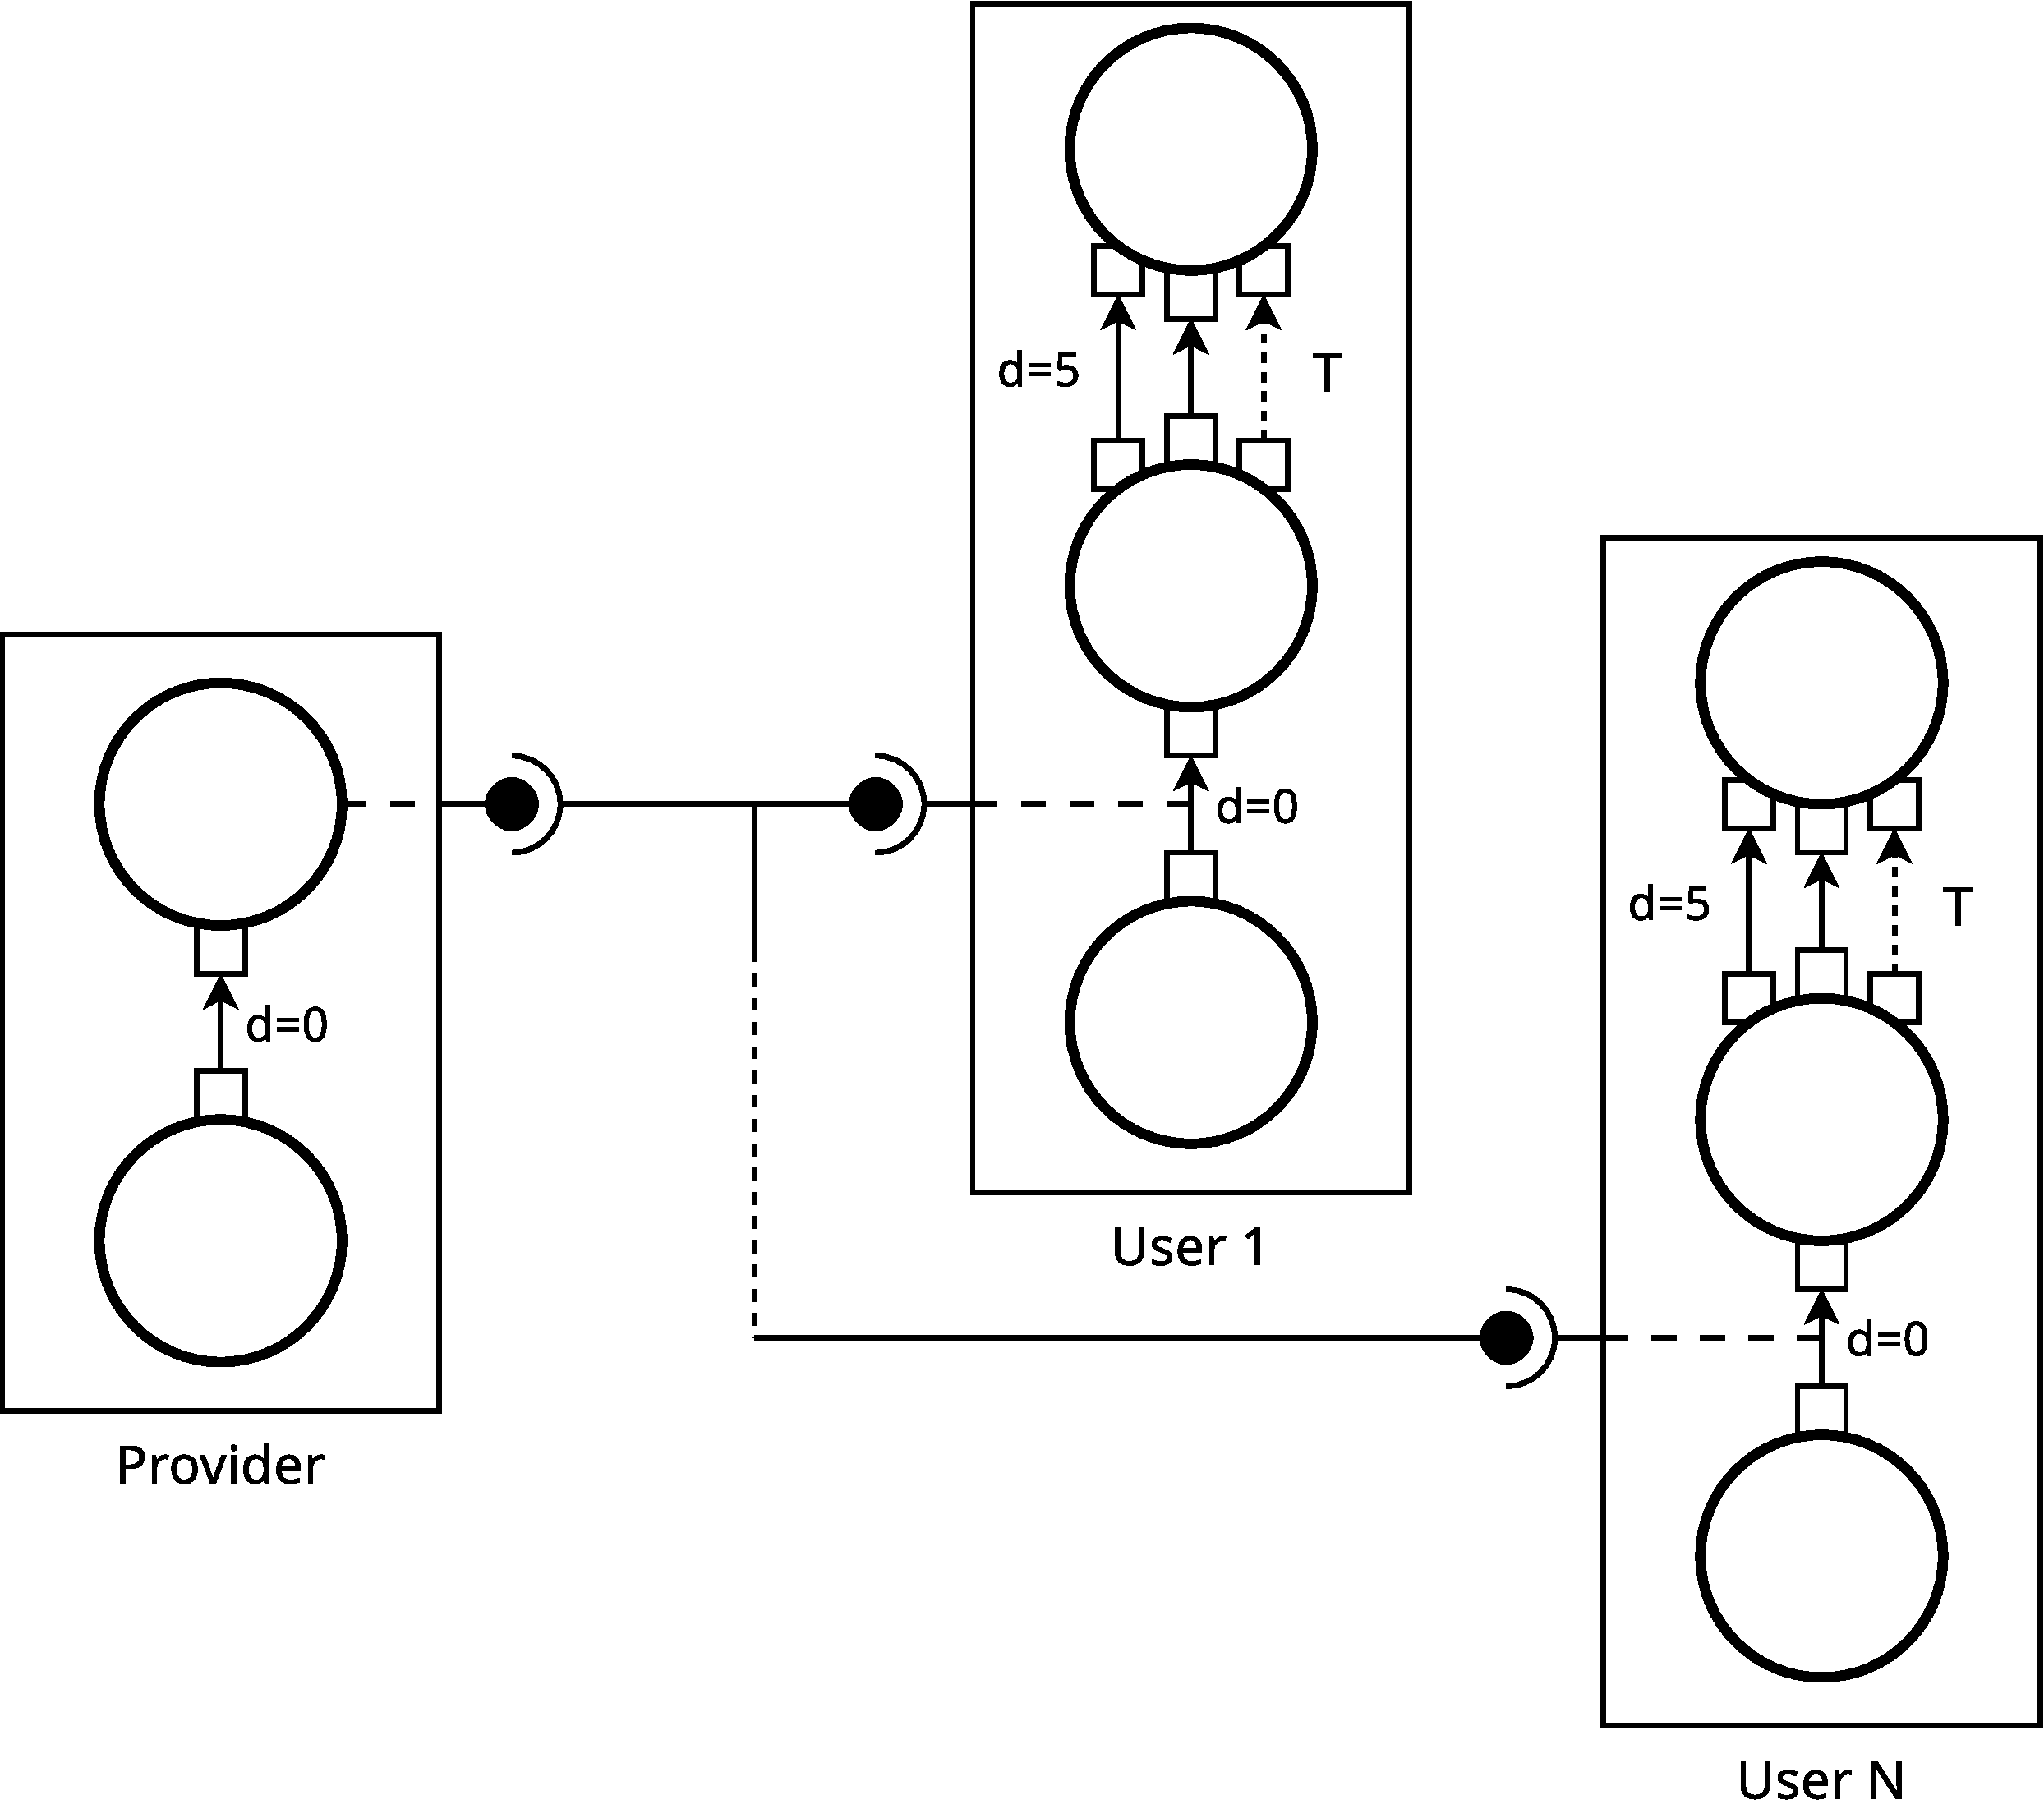
\includegraphics[width=0.4\textwidth]{./images/par.pdf}
    \caption{The \mad parallel assembly of Benchmark (B) and (C), with N parallel components, and T parallel transitions. The dotted connection represents that $N$ other components exist in this assembly.}
    \label{fig:par}
  \end{center}
\end{figure}

%second
The two other benchmarks model \mad parallel assemblies and are
depicted in Figure~\ref{fig:par}. The first assembly, denoted (B)
evaluates parallelism at the component level, called \emph{inter-comp}
and \emph{inter-comp-tasks}. The second one, denoted (C), evaluates
parallelism at the transition level, \ie \emph{intra-comp-tasks}, when
transitions are performed simultaneously.
%
Both benchmarks use the same assembly that is composed of an initial
\emph{provider} component and $N$ parallel \emph{user} components
connected to the provider. Each \emph{user} component contains a first
transition that uses the service provided by the provider component
and $T$ parallel transitions. For Benchmark (B), the number of
components varies from 1 to 40 components with a single transition per
component $T=1$. For Benchmark (C), the number of components is fixed
to $N-1=1$ and the number of transitions varies from 1 to 40.

Experiments have been performed on a single node of the \ecotype
cluster of the experimental platform
Grid'5000\footnote{\url{www.grid5000.fr}}. The detailed configuration
of the node is given in Table~\ref{tab:g5k}. Each experiment presented
in the results is an average of ten executions. The duration of some
transitions of the benchmarks are set to $d=0$ and the transitions
that are interesting for the results are set to $d=5$ (seconds). This
execution time is guaranteed by a call to the sleep function of
\python. This execution time has been chosen to get a coherent and
readable scale of results.
%They are both evaluated in \emph{dryrun} mode without any
%ssh connections and with \emph{ssh connections} active in the assembly
%between components, so as to allow visualisation of the eventual
%overhead of having these ssh connections.

%\begin{figure}[h]
%  \begin{center} 
%    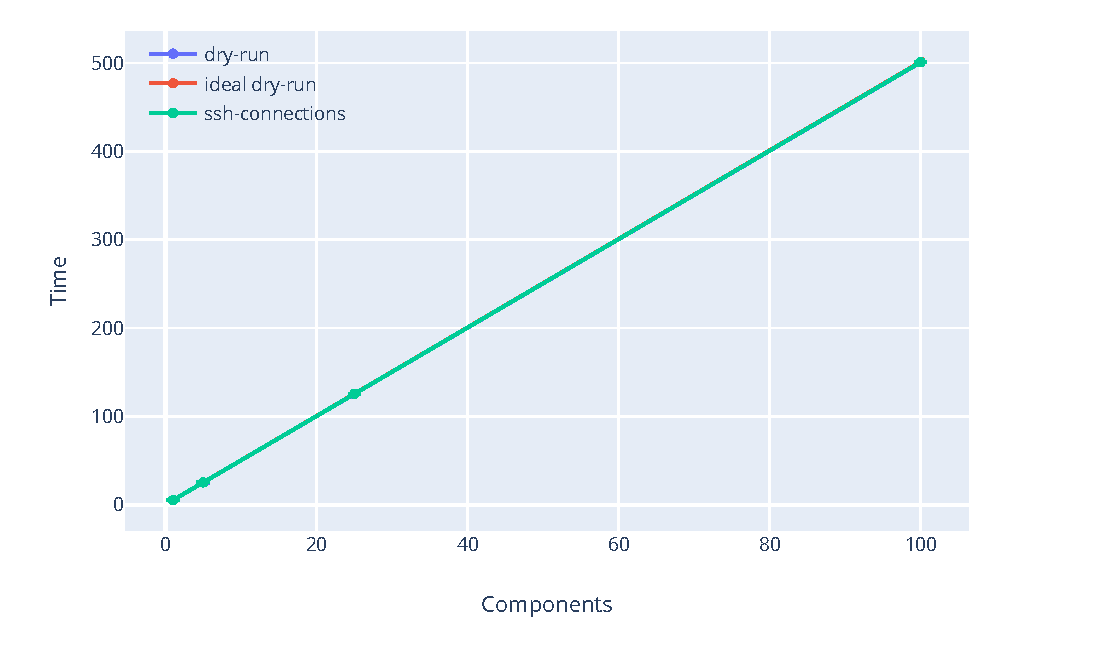
\includegraphics[width=0.5\textwidth]{./images/evaluations_sequential.pdf}
%    \caption{Results of the sequential benchmark.}
%    \label{fig:seqres}
%  \end{center}
%  \CP{En plus, plot ratio of two curves ? -- là on n'en voit qu'une}
%\end{figure}

Table~\ref{tab:resultssynt} presents the results of Benchmarks (A),
(B) and (C) with the theoretical execution time, the measured
execution time as well as its standard deviation, and the proportional
difference between them. As (A) models a sequential assembly, the
theoretical execution time is simply the sum of the execution time of
each transition of each component ($N$ components).
%
 
%The results show a linear increase in time and the \emph{dryrun} curve follows the \emph{ideal} curve closely.
%The difference between the
%\emph{ssh-connections} curve is hard to visualise but is slightly
%higher than the \emph{ideal} and \emph{dryrun} curves, a logical
%result as the number of ssh connections grows with each component
%added, but there is always only one ssh connection at the same time.

%\begin{figure}[h]
%  \begin{center} 
%    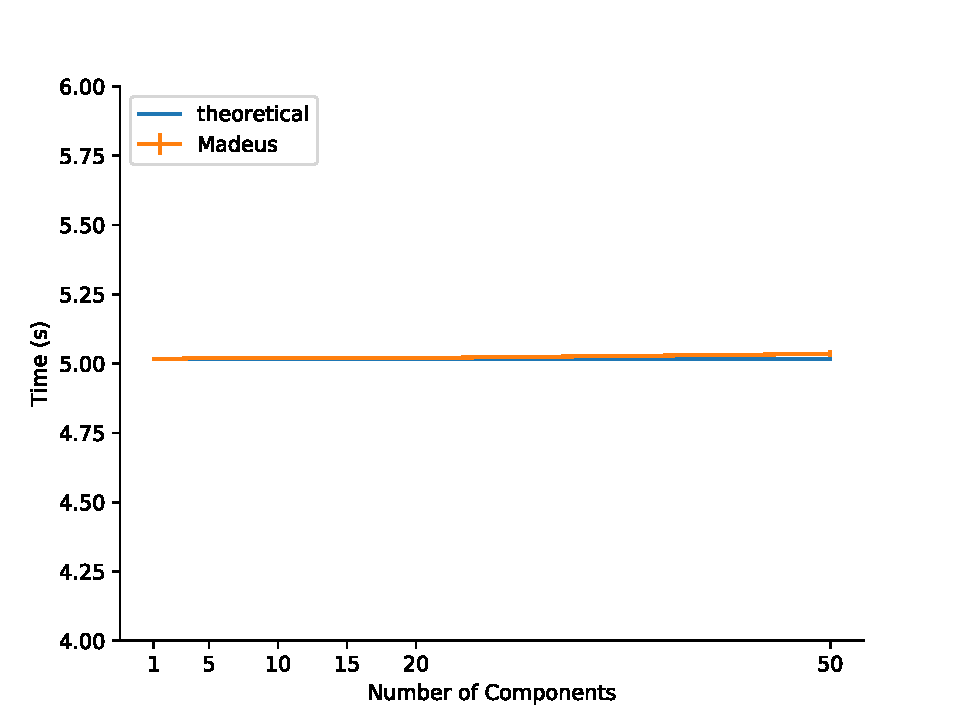
\includegraphics[width=0.5\textwidth]{./images/evaluations_par_component.pdf}
%    \caption{Results of the parallel assembly benchmark with varying component number}
%    \label{fig:parcompres}
%  \end{center}
%\end{figure}

% attention à comprendre si c'est systématique !
%For the results on the parallel assembly benchmark, we had to remove
%one outlier data point on the parallel assembly benchmark for
%component parallelism, as the first iteration of the assembly with
%just one component always had 4 seconds added to the time and we could
%not pinpoint the exact reason for that. As it did not occur for any of
%the other iterations, we did not take it into account on the curve
%drawing for our Figure~\ref{fig:parcompres}. In the results directory
%that can be found on our repository we have included the original
%times.json and the modified times.json files to keep the original
%results intact.

For Benchmark (B), the ideal theoretical performance is constant, and
equal to the duration of the main transition of \emph{user}
components, \ie $5$ seconds. Indeed as components are independent from
each other (no ports) they are deployed simultaneously.
%value as components are commissioned in parallel. In \emph{dryrun}
%our experimental benchmark
%The \emph{ssh connection} curve allows us to see
%that there is steady increase of time, adding almost 3 seconds to the
%assembly deployment when reaching 40 parallel components. This show
%that the overhead added by the SSH connections is not null.

%\begin{figure}[h]
%  \begin{center} 
%    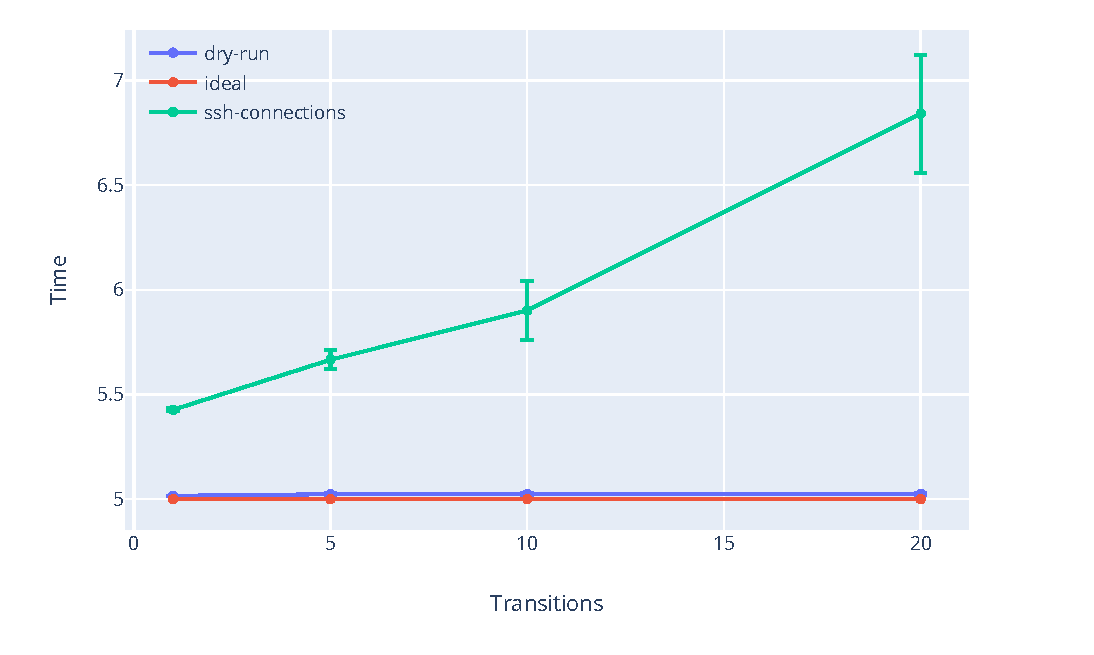
\includegraphics[width=0.5\textwidth]{./images/evaluations_par_transitions.pdf}
%    \caption{Results of the parallel assembly benchmark with varying parallel transition number}
%    \label{fig:partrans}
%  \end{center}
%\end{figure}

\begin{table}
	\begin{center}
		
\begin{tabular}{clc|ccc}
\toprule
& & & theory(s) & measured(s) & diff \\

\midrule
\multirow{5}{*}{(A)} & \multirow{5}{*}{\STAB{\rotatebox[origin=c]{90}{components}}} & 1 &
5 &
$5.015 \pm 0.021 \%$ &
0.3\% \\
 & & 10 &
50 &
$50.11 \pm 0.0004 \%$ &
0.22\%\\
 & & 20 &
100 &
$100.21 \pm 0.0004 \%$ &
0.21\%\\
 & & 30 &
150 &
$150.316 \pm 0.0003 \%$ &
0.21\% \\
& & 40 &
200 &
$200.42 \pm 0.0009\%$ &
0.21\% \\
\cmidrule{2-6}\multirow{5}{*}{(B)} & \multirow{5}{*}{\STAB{\rotatebox[origin=c]{90}{components}}} & 1  &
5 &
$5.016 \pm 0.0049\%$ &
0.32\% \\
& & 10 &
5 &
$5.021 \pm 0.1\%$ &
0.42\%\\
& & 20 &
5 &
$5.026 \pm 0.12\%$ &
0.53\%\\
& & 30 &
5 &
$5.028 \pm 0.068\%$ &
0.56\% \\
& & 40 &
5 &
$5.03 \pm 0.073 \%$ &
0.6\% \\
\cmidrule{2-6}\multirow{5}{*}{(C)} & \multirow{5}{*}{\STAB{\rotatebox[origin=c]{90}{transitions}}} & 1  &
5 &
$5.016 \pm 0.0057\%$ &
0.32\% \\
& & 10 &
5 &
$5.024 \pm 0.094\%$ &
0.48\%\\
& & 20 &
5 &
$5.025 \pm 0.06\%$ &
0.5\%\\
& & 30 &
5 &
$5.029 \pm 0.098\%$ &
0.58\% \\
& & 40 &
5 &
$5.033 \pm 0.136\%$ &
0.66\% \\
\bottomrule
\end{tabular}
		\caption{Theoretical and measured results of our three synthetic 
		benchmarks on \ecotype. The difference between the measured and expected 
		theoretical time is represented as a percentage.}
		\label{tab:resultssynt}
	\end{center}
\end{table}

Similarly, for Benchmark (C), because transitions are executed
simultaneously, the theoretical expected time is constant, and equal
to the duration of one of the $T$ transitions, \ie $5$ seconds.

For all benchmarks, results on the \mad prototype are only slightly
superior to the ideal theoretical result, showing that the prototype
does not add significant overhead to the process even for a large
number of sequential components, parallel components and parallel
transitions on the same node.  We may have increase the number of
components and transitions but we claim that 40 parallel transitions
and 40 components on a single node is already beyond normal usage when
deploying distributed software systems.

%calculation for the ideal curve on the parallel assembly benchmark
%when varying the number of parallel transitions has been done in the
%same manner as for the parallel component variation. In \emph{dryrun}
%the benchmark results follow the ideal curve closely as well, whereas
%the \emph{ssh connections} curve has an overhead that grows as the
%number of transitions increases.

These results allow us to point out that \mad does not by itself add a
significant overhead to the deployment --- at most 40 milliseconds in
these synthetic experiments. Note however that according to the
type of commands performed in the transitions, an additional overhead
could be observed. For instance, a high number of simultaneous SSH
connections could add an important overhead. In the experiments
presented in this paper, this problem is handled by using Ansible
within actions. Indeed, Ansible optimizes the number of SSH
connections on a single host, limiting the impact of this issue.
%They also show the
%importance of ssh connection and their impact on the deployment time.


